\documentclass[11pt]{beamer}
\usepackage[utf8]{inputenc}
\usepackage[T1]{fontenc}
\usepackage{lmodern}
\usetheme{Rochester}
\usepackage{graphicx}
\begin{document}
	\title{\textbf{Website Design Ranker}}
	\subtitle{Using Machine Learning}
	%\logo{}
	\institute{\large Department of Computer Science and Engineering \\\textbf{FISAT}}
	\date{16 SEPTEMBER 2019}
	\author{{\scriptsize Adhyaksh Guhan - 7 , Anet Eliza Johny - 23 , Dharwish Raj - 47 , \\ Joel J Padayattil - 60}}
	%\setbeamercovered{transparent}
	%\setbeamertemplate{navigation symbols}{}
	\begin{frame}[plain]
		\maketitle
	\end{frame}
	\begin{frame}{Introduction}
		\begin{itemize}
			
			
			\item Our project is aimed at ranking websites in terms of its design which is evaluated baised on certain parameters.
			
			\item Since a perfect model for wedsite ranking  is not in practice this  follows ranking according to submissions by critics.
			
			\item Thus we compare ranking implementation done by Google that analyses a webpage's content.
		
			\item We will be comparing against:
				\item A Website that ranks other design according to submissions by critics
				\item A ranking implementation done by Google that analyses a web-page's contents
		\end{itemize}
	\end{frame}
	\begin{frame}{Problem Statement}
		\begin{itemize}

			\item Our main problem is to evaluate website designs using an algorithm that uses machine learning
			
			\item It must take into account various parts of the website to use as parameters.
			
			\item for example: pepole won't be intrested to visit a site if they are berated with adds.Thus adds above a degree will be considered as the parameter for ranking.

			\item There are no existing algorithms or methods that manage to analyze and evaluate websites in this way.
		\end{itemize}
	\end{frame}
	\begin{frame}{Why "Website Design Ranker" ?}
			\begin{itemize}
			\item Website Design Ranker will rank set of input websites based on certain parameters.
			\item It will be helpful to find best website among list of websites which have same content.
			\item We can compare our website design with other competing websites.
			\item We can see how a website's design may improve in an area.

			\end{itemize}
	\end{frame}
	\begin{frame}{Existing Methods : Website Design Ranking Agencies }
		\begin{itemize}
			\item Websites are ranked by Ranking Agencies as per submission on their database.
			\item Hired critics and analyzing staffs are reviewed and ranked according to their policy.
			\\\
			\\Example:\\
			https://www.awwwards.com\\

			https://www.cssdesignawards.com\\

			https://www.csswinner.com/winners\\

			https://thefwa.com\\
		\end{itemize}
	\end{frame}
	\begin{frame}
	\frametitle{{Existing Methods : Google Page Layout}}
	\begin{itemize}
		\item Google introduced Page Layout Algorithm to analyze website readability.[1]
		\item Looks for the layout of the web page and the amount of content we see in the page once we click on a result.[1]
		
		\item Focuses to reduce the difficulty of users to find the actual content.[1]
		
		\item  The websites which does not have a lot of visible content above-the-fold and dedicates a large fraction (above a normal degree) to ads will be affected.[1]
		
		
	\end{itemize}

	\end{frame}
	\begin{frame}
	\frametitle{{Existing Methods : Google Page Layout}}
		\begin{figure}
		
		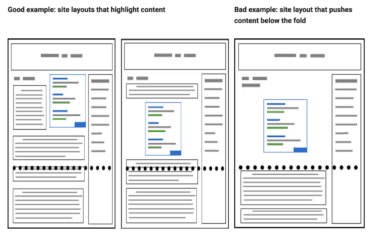
\includegraphics[width=10cm]{image/gpa.png}
		\caption{One of the criteria of GPL Algorithm\textsuperscript{[Fig:1]}}
		\label{fig1:gpa}
	\end{figure}
	\end{frame}
\begin{frame}
			\frametitle{{Comparison}}
	\begin{itemize}

		\item \textbf{Existing Methods : Website Design Ranking Agencies}
		\item Website design ranking agencies are not capable of analyzing particular website with different other websites.
		\item Ranking Varies from each critic or staff, cant be used in large scale, time consuming.
		\item \textbf{Existing Methods : Google Page Layout Algorithm}
		\item Only looking for layout of the page, more importance for SEO.
		\item Proprietary code of Google

	\end{itemize}
\end{frame}

\begin{frame}
\frametitle{{Problem Analysis}}
\begin{itemize}
	\item Our main effort was to create an algorithm for ranking websites baised on the parameters.Even a simple looking wedsites with exceptional usability and well-structured will cope up with the expectation of the users.
	
	\item This will allow users to deviate from the existing mannual ranking system of wedsites design.
\end{itemize}
\end{frame}



		\begin{frame}{What we proposed?}
			\begin{itemize}
				\item We propose a system where an algorithm scrubs through a website, looking for various elements.
				\item Once we discover the nature of these elements, we check whether the parameters we have set (eg: colour, symmetry, etc) have been met.
				\item For each parameter met, a website will obtain a mark.
				\item Once all parameters have been checked, the website receieves an overall score (the sum of all marks) that ranks its design.
					\end{itemize}	
	\end{frame}
	\begin{frame}{Conclusion}
		\begin{itemize}
			\item Here we can see the logical differences in the approaches that our algorithm takes versus any existing methods.
			\item Our method relies on an objective and automated method that is consistent in nature as opposed to the subjective methods of the existing methods.
		\end{itemize}
	\end{frame}
	\begin{frame}
		\frametitle{\LARGE \textbf{References}}
		\begin{itemize}
			\item [1] - Google Page Layout Algorithm: Everything You Need to Know 
			"https://www.searchenginejournal.com/google-algorithm-history/page-layout/close"
			\item [Fig:1] - https://cdn.searchenginejournal.com/wp-content/uploads/2017/10/google-algorithm-above-the-fold-380x238.png
		\end{itemize}
	\end{frame}
\end{document}
